\documentclass[11pt]{article}
\usepackage[T1]{fontenc}
\usepackage{latexsym,amssymb,amsmath,amsfonts,amsthm}
\usepackage{color}
\usepackage{tikz}
\usetikzlibrary{calc}
\usetikzlibrary{intersections,through}

\begin{document}

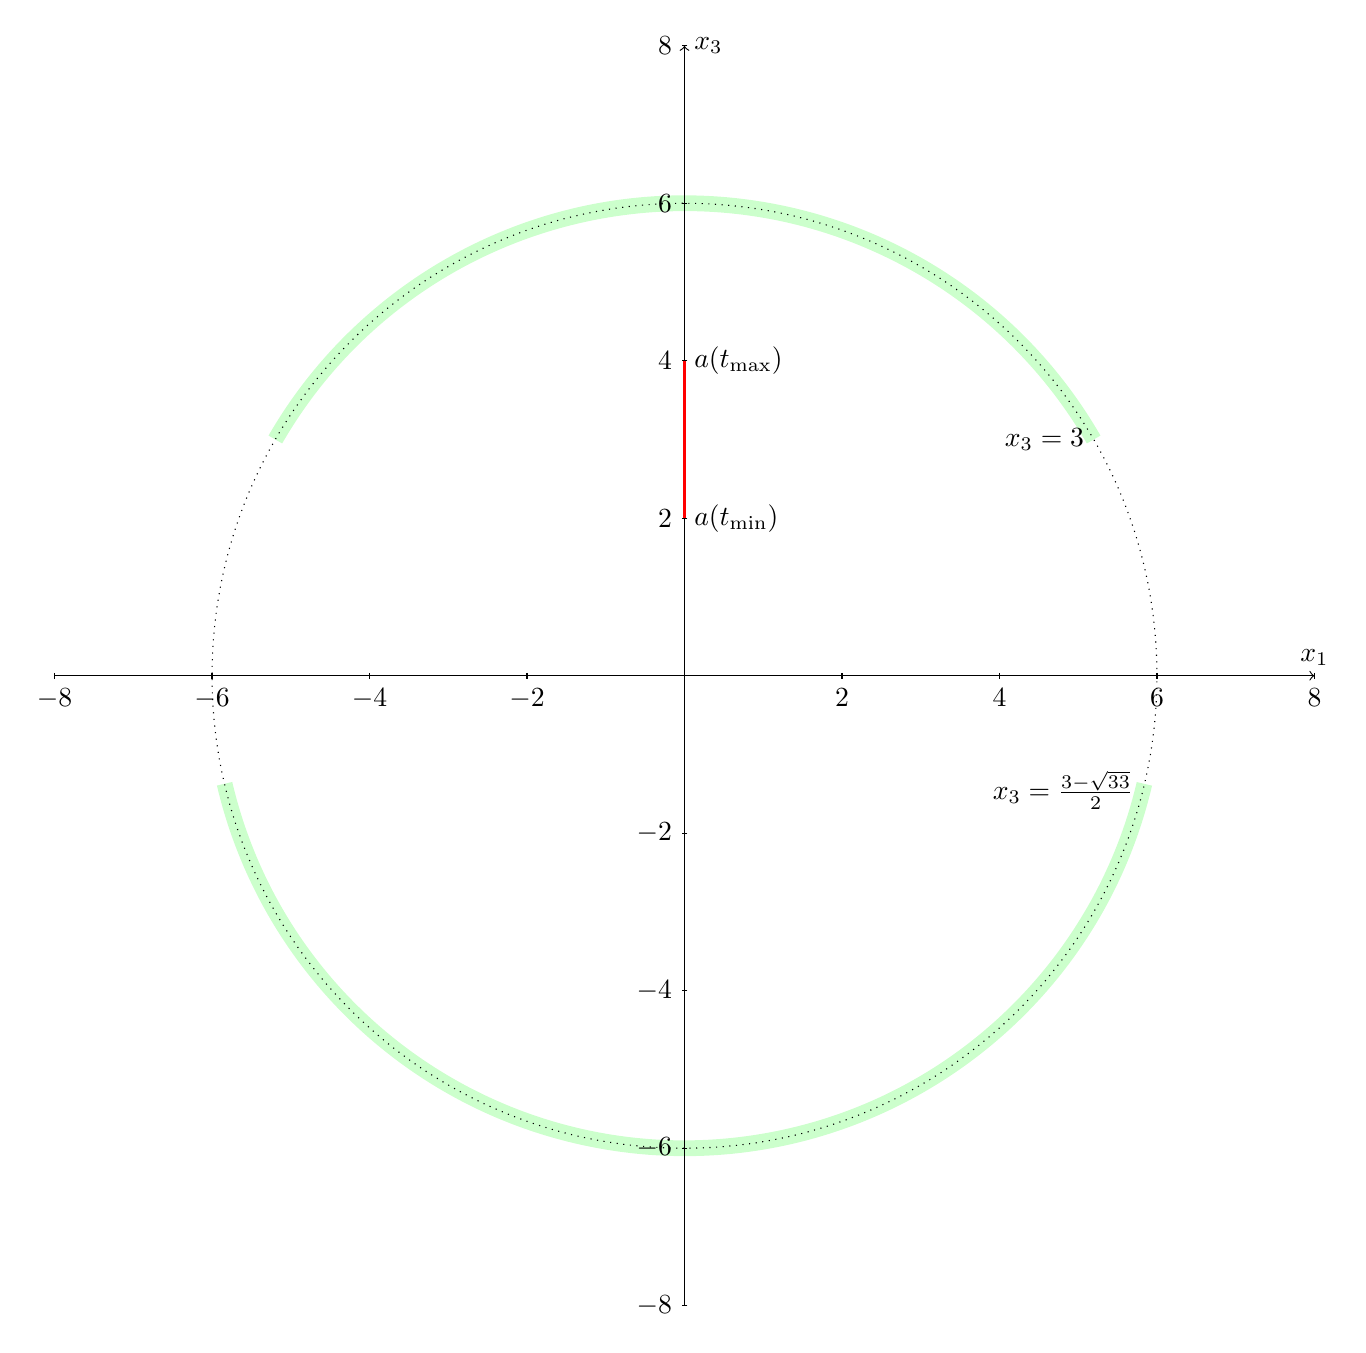
\begin{tikzpicture}
		\fill[green!20] (30:5.9) --(30:6.1) arc (30:150:6.1) --(150:5.9) arc (150:30:5.9);

		\fill[green!20] (346.77:5.9) --(346.77:6.1) arc (346.77:193.22:6.1) --(193.22:5.9) arc (193.22:346.77:5.9);




		\draw[->] (-8,0) -- (8,0) node[above] {$x_1$} coordinate(x axis);
		\draw[->] (0,-8) -- (0,8) node[right] {$x_3$} coordinate(y axis);
		\foreach \x/\xtext in {-8,-6,-4,-2, 2, 4, 6, 8}
		\draw[xshift=\x cm] (0pt,1pt) -- (0pt,-1pt) node[below] {$\xtext$};
		\foreach \y/\ytext in {-8,-6,-4,-2, 2, 4, 6, 8}
		\draw[yshift=\y cm] (1pt,0pt) -- (-1pt,0pt) node[left] {$\ytext$};

		\draw [dotted] (6,0) arc [ start angle = 0, end angle = 360, radius = 6];
		\draw [very thick,red] (0, 2) -- (0,4);

		\draw (0, 2) node [right] {$a(t_{\min})$};

		\draw (0,4) node [right] {$a(t_{\max})$};
		\draw (30:6) node [left] {$x_3=3$};
		\draw (346:6) node [left] {$x_3=\frac{3-\sqrt{33}}{2}$};

		\end{tikzpicture}

\end{document}